\documentclass[a4paper, 12pt]{article}
\usepackage{amsmath}
\usepackage[utf8]{inputenc}
\usepackage{graphicx}
\usepackage[left=2.5cm, right=2.5cm, bottom=2.5cm, top=2.5cm]{geometry}
\usepackage{natbib}
\usepackage{microtype}

\title{Measure --- or as the kids call it, addition}
\author{Brendon J. Brewer}
\date{}

\begin{document}
\maketitle

% Need this after the abstract
\setlength{\parindent}{0pt}
\setlength{\parskip}{8pt}

\section{Bigger and smaller}
Some things are bigger than others.

\section{How long is a piece of string?}

\section{The sum rule}

\section{Measure in boolean lattices}


\begin{figure}[!ht]
\centering
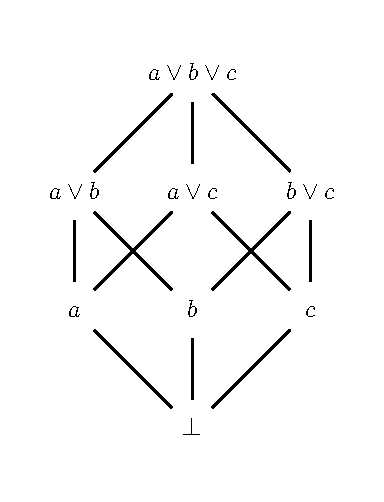
\includegraphics[width=0.5\textwidth]{figures/boolean_lattice.pdf}
\caption{\label{fig:boolean_lattice}}
\end{figure}


Apples.
One bag of apples combined with another bag of apples.
The exact same situation. The numbers of apples add, as
do the masses. Two different sum rules apply to the same
situation!


\section{Infidelity and ``signed measure''}

\subsection{A fate worse than death}

\end{document}

